%Implementaci\'on

\section{Dispositivos de desarrollo y despliegue}
\noindent Con el fin de desarrollar la herramienta se utiliz\'o un computador de mesa con las siguientes caracter\'isticas:
\begin{itemize}
        \item Computador \begin{itemize}
            \item \textbf{Tarjeta Gr\'afica:} GeForce RTX 3060
            \item \textbf{Procesador:} AMD Ryzen 5 3400G
            \item \textbf{RAM:} 16 GB
            \item \textbf{Almacenamiento:} 1 TB
        \end{itemize}
    \end{itemize}
\noindent Se eligi\'o trabajar con un computador que tuviern una buena tarjeta gr\'afica y procesador decente, para hacer del proceso de desarrollo m\'as fluido y sin complicaciones. 
\\
\\
\noindent Para hacer pruebas tambi\'en se utiliz\'o un celular:
\begin{itemize}
    \item Celular \begin{itemize}
        \item \textbf{Modelo: } Xiaomi Redmi Note 10
        \item \textbf{RAM: 8GB }
        \item \textbf{Procesador:} Snapdragon 732G
        \item \textbf{GPU:} Adreno 618 
        \item \textbf{C\'amara Frontal:} 16 MP, f/2.5
        
    \end{itemize}
\end{itemize}


\subsection{Proceso de conectar Python con R} 
\noindent El proyecto Foodprice es un proyecto de la Pontificia Universidad Javeriana Cali que busca generar un sistema que permita a las personas en condici\'on de pobreza generar una dieta de costo m\'inimo que se adapte a sus necesidades nutricionales, as\'i como a sus caracter\'isticas f\'isicas. Sin embargo dicho proyecto presenta una complicaci\'on, al estar desarrollado en el lenguaje R, es muy poco accesible para la poblaci\'on en general, y menos a\'un para las poblaciones de escazos recursos, esto debido a que estadisticamente estas poblaciones son m\'as propensas a tener bajo nivel de escolaridad [referencia], por lo que un software que requiera conocimiento t\'ecnico alto para usarse, ser\'a complicado que logre tener un impacto.
\\
\\
Por este motivo, se crea este proyecto. Sin embargo, en su desarrollo tambi\'en se presentan diversos obst\'aculos. Esto debido a que se quiere poder consumir el paquete en R de Foodprice a trav\'es de un lenguaje m\'as moderno y con un gran alcance como lo es Python. Pero, lograr comunicar de forma fluida y eficiente aplicaciones construidas en lenguajes diferentes no resulta ser una tarea f\'acil, por lo que se opt\'o por convertir el paquete de Foodprice en una API, para as\'i interactuar de estar forma con una API en python, la cual le pase una entrada, que el paquete en R utilice para calcular la dieta de costo m\'inimo adecuada a sus necesidades. Para poder lograr esto, se tuvo que modificar tambi\'en el paquete en R, para recibir par\'ametros externos y calcular las dietas con normalidad. Adem\'as de esto, se utiliz\'o el paquete Plumber para lograr convertir Foodprice en una API, y se utiliz\'o FastAPI en Python para crear la API de python que se encargar\'a de llamar al proyecto Foodprice y enviarle los par\'ametros para que funcione adecuadamente.





\subsection{Retos de implementaci\'on backend (Web Scraping)}
\noindent Ya que el paquete Foodprice realiza c\'alculos de dietas basado en precios mayoristas aportados por el Departamento Administrativo Nacional de Estad\'istica, dichos datos no reflejan de manera acertada los precios a granel de una dieta que un ciudadano com\'un podr\'ia encontrar en un supermercado. Con la finalidad de contrarrestar esta falencia, se decidi\'o emprender un proyecto de web scraping en el supermercado Almacenes \'Exito; donde se busc\'o obtener la informaci\'on de m\'ultiples productos que se encontraran listados en el sistema de Gu\'ias Alimentarias Basadas en Alimentos (GABAS) del Instituto Colombiano de Bienestar Familiar.
\\
\\
Esto debido a  que el GABAS provee los datos nutricionales de los alimentos, con lo cual al obtener los productos de un supermercado com\'un y cruzar la informaci\'on con esta base de datos, se obtendr\'ia un mejor estimado en cuanto a la nutrici\'on que se puede obtener por cada peso que se invierte en la alimentaci\'on de distintos grupos poblacionales. Sin embargo, no siempre los nombres de los productos en GABAS o SIPSA se corresponden a los nombres coloquiales o comunes por los cuales se consiguen en los supermercados. Tomemos como ejemplo el producto con identificador C079 en la base de datos SIPSA, este producto tiene el nombre de ``Patilla'', sin embargo el uso de este nombre no es tan com\'un como el de ``Sand\'ia'', motivo por el cual si se realizara un proceso de web scraping sin cuidado, se podr\'ia llegar a casos en los que no se encuentre informaci\'on de ciertos productos cuando simplemente buscando con otros nombres estos aparecer\'ian.
\\
\\
Una vez identificada esta problem\'atica, es claro que se tiene que realizar un proceso de verificaci\'on de los datos obtenidos por el sistema de web scraping con la finalidad de obtener y pulir la mayor cantidad de datos posible; esta verificaci\'on manual puede resultar exhaustiva, pero vale la pejna cuando se piensa en la meta de generar dietas con datos precisos y realistas, que suplan las necesidades de poblaciones econ\'omicamente vulnerables por el menor costo posible.





\subsection{Retos implementaci\'on frontend} 
\noindent Ya que el proyecto tiene como objetivo ofrecer un sistema accesible para el c\'alculo de dietas, se tiene que asegurar que el sistema se adapte bien a todo tipo de pantallas, desde las m\'as peque\~{n}as hasta las m\'as grandes, lo cual supone un reto cuando se quiere contar a la vez con un sistema agradable a la vista. 
\\
\\
Otro factor clave para este proyecto era la poblaci\'on objetivo, los cuales al encontrarse en situac i\'on de pobreza, tienen mayor probabilidad de no tener acceso a un alto nivel eduativo, tecnolog\'ia de alta gama, o un internet de alta velocidad. Debido a esto se prioriz\'o que el dise\~no final de la aplicaci\'on fuera simple, sin tantos elementos cargados que puedan confundir, con una navegaci\'on directa, y con textos que acompa\~nen y expliquen las funcionalidades del sistema.
\\
\\
Con todo esto,  la aplicaci\'on final se observa a continuaci\'on:


\begin{figure}[H]
    \centering
    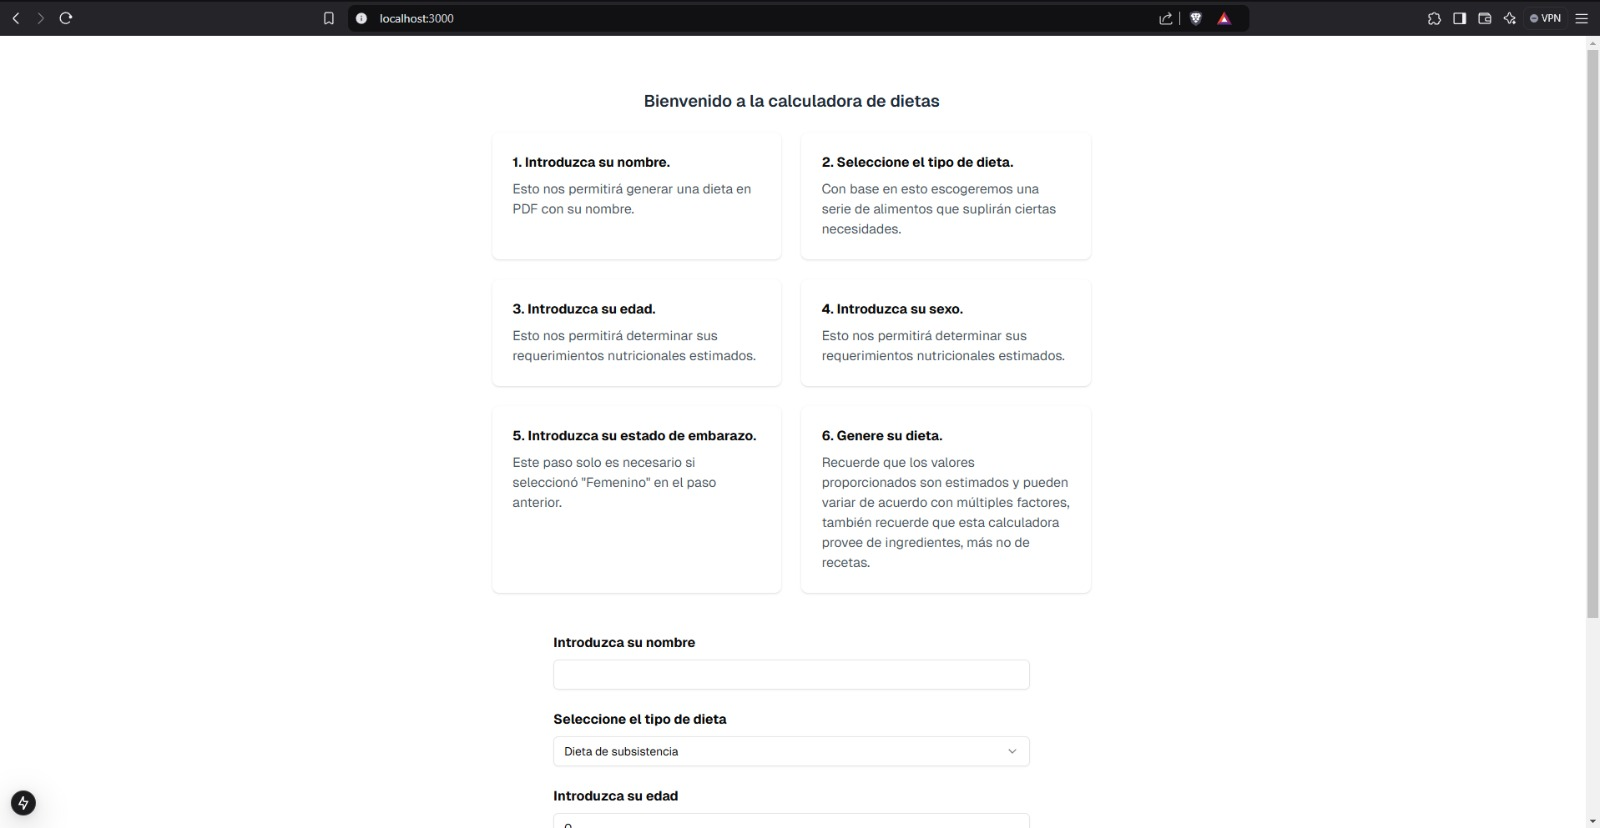
\includegraphics[width=15cm]{img/implementacion/implementacion.jpeg}
    \caption{implementaci\'on del sistema 1}
    \label{fig:implementacion1}
\end{figure}

Como se puede observar en la figura \ref{fig:implementacion1}, es la vista inicial que se tiene del sistema al utilizarlo en PC, aqu\'i se puede observar como un factor importante es dar instrucciones claras, para que el usuario entienda que hacer, y sepa tambi\'en que esperar

\begin{figure}[H]
    \centering
    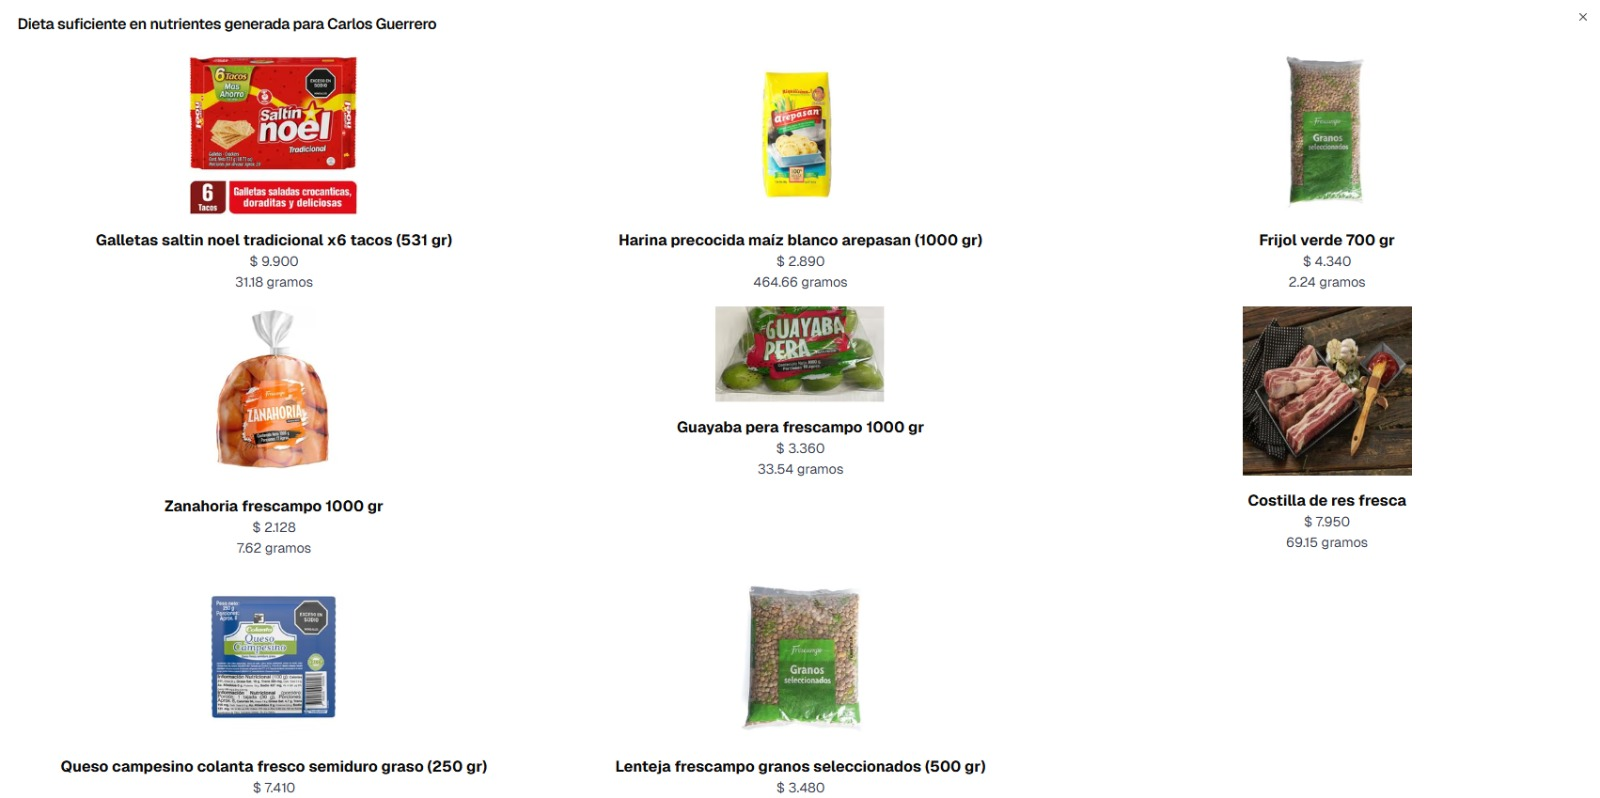
\includegraphics[width=15cm]{img/implementacion/implementacion5.jpeg}
    \caption{implementaci\'on del sistema 2}
    \label{fig:implementacion2}
\end{figure}

De la misma forma se observa en la figura \ref{fig:implementacion2}, la vista de una dieta ya generada, adaptada a las necesidades del usuario, en la cual destaca el uso de im\'agenes para mostrar los alimentos, con lo cual se puede realizar una asociaci\'on m\'as directa a trav\'es de la vista que  solo al leer una lista de productos. Se observa tambi\'en como se ve directamente toda la informaci\'n relevante respecto a cada producto, y adem\'as si se presiona cualquiera de los productos, dirige al link para comprar dicho producto.


\begin{figure}[H]
    \centering
    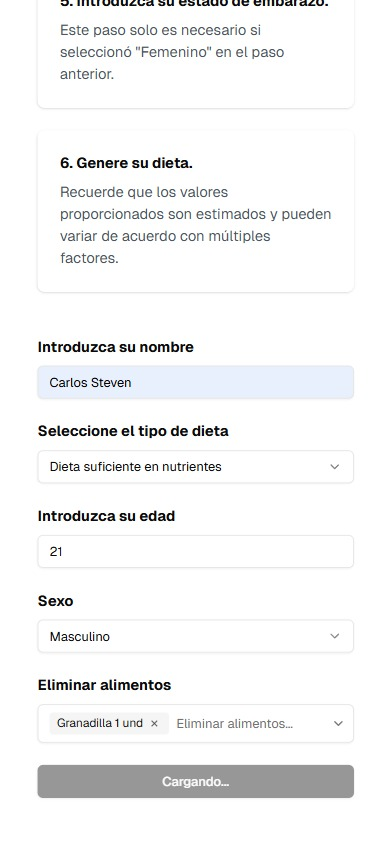
\includegraphics[height=10cm]{img/implementacion/implementacion4.jpeg}
    \caption{implementaci\'on del sistema 3}
    \label{fig:implementacion3}
\end{figure}

En comparaci\'on, se tiene tambi\'en en la figura \ref{fig:implementacion3} la aplicaci\'on al verla desde un tel\'efono movil, con lo cual a pesar de que cambian las dimensiones, se sigue manteniendo la est\'etica del proyecto, adem\'as de que se conservan los elementos m\'as importantes, la informaci\'on para generar una buena experiencia de usuario.

\begin{figure}[H]
    \centering
    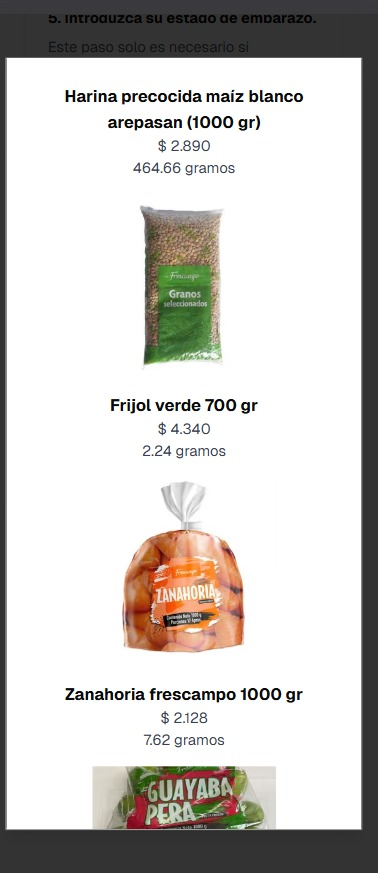
\includegraphics[height=10cm]{img/implementacion/implementacion2.jpeg}
    \caption{implementaci\'on del sistema 4}
    \label{fig:implementacion4}
\end{figure}

\begin{figure}[H]
    \centering
    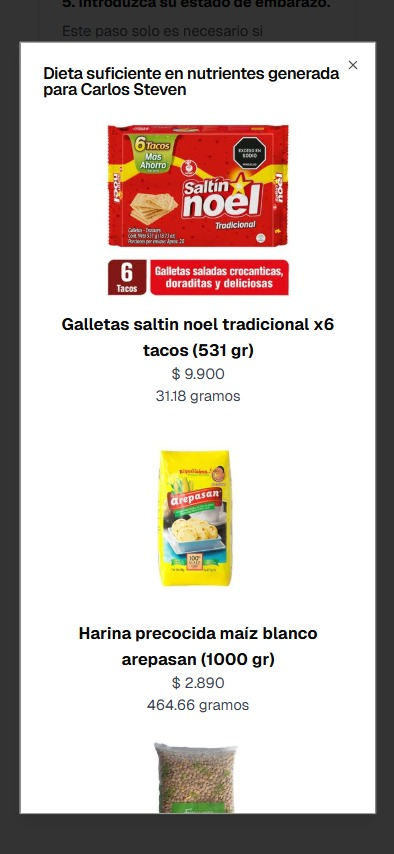
\includegraphics[height=10cm]{img/implementacion/implementacion3.jpeg}
    \caption{implementaci\'on del sistema 5}
    \label{fig:implementacion5}
\end{figure}


